\documentclass[11pt]{article}
\usepackage{latexsym}
\usepackage{amsmath}
\usepackage{amssymb}
\usepackage{amsthm}
\usepackage{epsfig}
\usepackage[tight]{subfigure}

\usepackage{amsmath}

\DeclareMathOperator*{\minimize}{min}
\DeclareMathOperator*{\maximize}{max}

\usepackage{algorithm}
 %on linux you may need to run sudo apt-get install texlive-full to install algorithm.sys
\usepackage{algorithmic}

\usepackage{verbatim}
\usepackage{amsmath,amsfonts,amsthm,bm}

\newcommand{\handout}[5]{
  \noindent
  \begin{center}
  \framebox{
    \vbox{
      \hbox to 5.78in { {#1} \hfill #2 }
      \vspace{4mm}
      \hbox to 5.78in { {\Large \hfill #5  \hfill} }
      \vspace{2mm}
      \hbox to 5.78in { {\em #3 \hfill #4} }
    }
  }
  \end{center}
  \vspace*{4mm}
}

\newcommand{\lecture}[5]{\handout{#1}{#2}{#3}{#4}{#5}}
\newcommand{\collision}[0]{\mathrm{collision}}
\newcommand{\nocollision}[0]{\overline{\collision}}

\newcommand*{\QED}{\hfill\ensuremath{\square}}

\newtheorem{theorem}{Theorem}
\newtheorem{corollary}[theorem]{Corollary}
\newtheorem{lemma}[theorem]{Lemma}
\newtheorem{observation}[theorem]{Observation}
\newtheorem{proposition}[theorem]{Proposition}
\newtheorem{definition}[theorem]{Definition}
\newtheorem{claim}[theorem]{Claim}
\newtheorem{fact}[theorem]{Fact}
\newtheorem{assumption}[theorem]{Assumption}
\newtheorem{note}[theorem]{Note}

% 1-inch margins, from fullpage.sty by H.Partl, Version 2, Dec. 15, 1988.
\topmargin 0pt
\advance \topmargin by -\headheight
\advance \topmargin by -\headsep
\textheight 8.9in
\oddsidemargin 0pt
\evensidemargin \oddsidemargin
\marginparwidth 0.5in
\textwidth 6.5in

\parindent 0in
\parskip 1.5ex
%\renewcommand{\baselinestretch}{1.25}

\begin{document}

\lecture{Statistical Techniques in Robotics (16-831, S22)}{Lecture \#08
  (Monday, February 14)}{Lecturer: Kris Kitani}{Scribes: Dakshit Agrawal, Lulu Ricketts}{Online Mirror Descent}

\section{Review}
%This section serves as a review of the previous lecture and any other context required to frame the content of the current lecture. 

%You may format the scribes in any way you like, aside from changing font style, size and page format. Please use subsections and paragraphs to increase the readability of your notes.

%Length requirement 1-2 pages.
In the previous lectures, we studied general online optimization algorithms. Recall that online optimization consisted of the following steps:

\begin{enumerate}
    \item Predict the weights $\textbf{w}^{(t)}$ (parameters) .
    \item Receive the loss function $f^{(t)}$ from nature.
    \item Compute the loss $f^{(t)}(\textbf{w}^{(t)})$ using the predicted weights $\textbf{w}^{(t)}$ and given loss function $f^{(t)}$.
\end{enumerate}

In particular, we read about the following two algorithms:
\begin{enumerate}
    \item Follow the Leader (FTL)
    \item Follow the Regularized Leader (FTRL)
\end{enumerate}

We also derived the regret bounds of these algorithms for linear and quadratic convex loss functions with weights in the convex space.

\subsection{Follow the Leader (FTL)}

The core principle of FTL is to choose those weights that have given the lowest loss till now (see Algo. \ref{algo:ftl}). 

\begin{algorithm}[H]
\caption{Follow the Leader (FTL)}
\label{algo:ftl}
\begin{algorithmic}[1]
\FOR{$t=1,2,\;\ldots,\;T$}

\STATE $\textbf{w}^{(t)} = \text{arg} \min\limits_{\textbf{w}\in W} \sum_{i=1}^{t-1} f^{(i)}(\textbf{w})$
\STATE \textsc{Receive} ($f^{(t)}: W \rightarrow \mathbb{R}$)
\ENDFOR
\end{algorithmic}
\end{algorithm}

We derived the regret bounds of FTL for the following convex functions:
\begin{enumerate}
    \item Linear Loss ($f^{(t)}(w) = wz^{(t)}$):
    \begin{itemize}
        \item Regret is $O(T)$
        \item The algorithm can be unstable in certain cases leading to its failure.
    \end{itemize}
    \item Quadratic Loss ($f^{(t)}(w) = \frac{1}{2} \Vert w - z^{(t)} \Vert_{2}^{2}$): 
    \begin{itemize}
        \item Regret $\leq 4L^{2}\left( \log(T) + 1 \right)$
        \item No regret!
        \item Stability in algorithm due to weight updates via averaging.
    \end{itemize}
\end{enumerate}

\subsection{Follow the Regularized Leader (FTRL)}

The core principle of FTRL is to ensure stability on weight prediction by adding a regularization term $\psi$ to the weight prediction step (see Algo. \ref{algo:ftrl}). FTL is a specific case of FTRL in which $\psi = 0$. 

\begin{algorithm}[H]
\caption{Follow the Regularized Leader (FTRL)}
\label{algo:ftrl}
\begin{algorithmic}[1]
\FOR{$t=1,2,\;\ldots,\;T$}

\STATE $\textbf{w}^{(t)} = \text{arg} \min\limits_{\textbf{w}\in W} \sum_{i=1}^{t-1} f^{(i)}(\textbf{w}) + \psi(\textbf{w})$
\STATE \textsc{Receive} ($f^{(t)}: W \rightarrow \mathbb{R}$)
\ENDFOR
\end{algorithmic}
\end{algorithm}

Taking a convex linear loss function like we did for FTL ($f^{(t)} = w \cdot z^{(t)}$), but now using a convex quadratic regularizer ($\psi(w) = \frac{1}{2\eta} \Vert w \Vert_{2}^{2}$), we get the regret bound of FTRL to be:


\centerline{$R^{(T)}(\textbf{u}) \leq BL\sqrt{2T}$}

where

\centerline{$L = \max\limits_{\textbf{z}} \Vert \textbf{z} \Vert_2$}

\centerline{$B = \max\limits_{\textbf{u} \in S} \Vert \textbf{u} \Vert_2$}

The solution space S is a convex set. As can be seen, the regret for a convex linear loss function is now \textbf{no regret} due to the quadratic regularizer.

Using online convex optimization, the stability of FTRL is generalized to:

\begin{itemize}
    \item any sequence of Lipschitz loss functions (not just linear)
    \item other convex regularization functions (not just quadratic)
\end{itemize}

Thus, regularization can be used to ensure stability and no-regret properties.

\section{Summary}
We will first look at how FTRL can be interpreted as Online Mirror Descent (OMD) (Sec. \ref{sec:omd}. Afterwards, we will build our geometrical intuition and mathematical understanding of duality (Sec. \ref{sec:duality}) to finally calculate the regret bound for OMD (Sec. \ref{sec:regret}).

\begin{figure}[H]
    \centering
    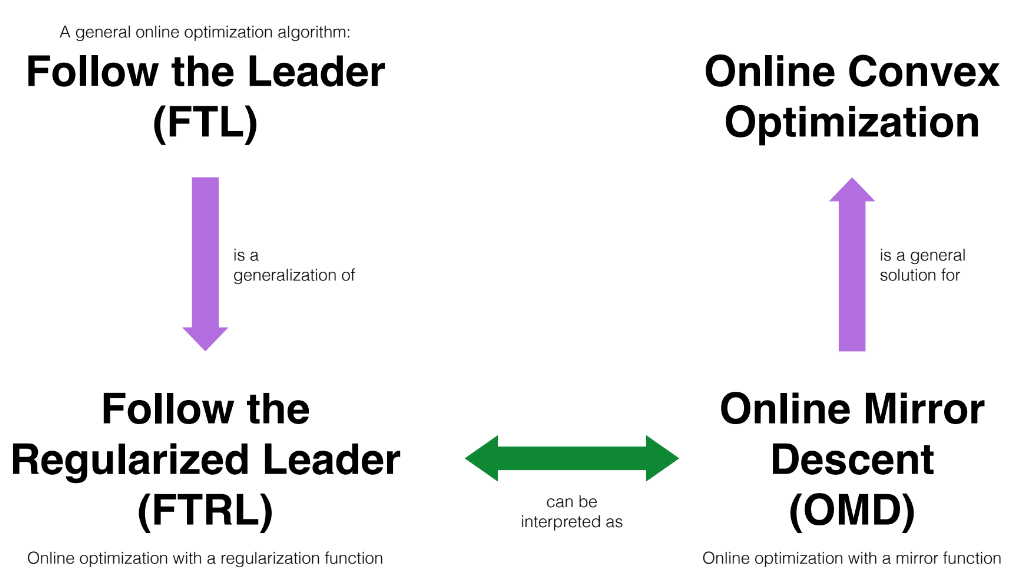
\includegraphics[width=0.7\textwidth]{figs/chart.png}
    \caption{Overview of how topics taught till now connect to each other}
    \label{fig:chart}
\end{figure}

\subsection{Online Mirror Descent (OMD)}
\label{sec:omd}

OMD provides another way to interpret FTRL when using a linear loss and convex regularizer. You might ask why we need this different perspective, since FTRL is stable and getting the job of online convex optimization done for us. The reason is two-fold:

\begin{itemize}
    \item provides a unification of online learning algorithms
    \item more mathematical tools for regret analysis
\end{itemize}

In the subsequent subsections, we will generalize FTRL with linear loss ($f^{(i)}(\textbf{w}) = \langle \textbf{w}, \textbf{z}^{(i)} \rangle$) to derive OMD.

\subsubsection{Generalize FTRL linear loss parameter sum}

The FTRL linear loss parameter sum is:
\begin{align}
\label{eq:1}
  \sum_{i=1}^{t} f^{(i)}(\textbf{w})
\end{align}

The gradient of Eq. \ref{eq:1} with respect to the parameters $\textbf{w}$ is:
\begin{align}
\label{eq:2}
    \textbf{z}^{(1:t)} = \sum_{i=1}^{t} \textbf{z}^{(i)}
\end{align}

Substituting $ \textbf{z}^{(1:t)}$ in Eq. \ref{eq:2} with a function of $\bm{\theta}^{(t+1)}$, where $\bm\theta$ a \textbf{parameter of the dual space}:
\begin{align}
\label{eq:3}
    \bm{$\theta$}^{(t+1)} \triangleq  - \textbf{z}^{(1:t)}
\end{align}

Using Eq. \ref{eq:2} and Eq. \ref{eq:3}, we get:
\begin{align*}
    \bm{$\theta$}^{(t+1)} &= - \sum_{i=1}^{t} \textbf{z}^{(i)}\\
    \bm{$\theta$}^{(t+1)} &= - \sum_{i=1}^{t-1} \textbf{z}^{(i)} - \textbf{z}^{(t)}\\
    \bm{$\theta$}^{(t+1)} &= - \textbf{z}^{(1:t-1)} - \textbf{z}^{(t)}
\end{align*}

Using Eq. \ref{eq:3}:
\begin{align}
\label{eq:4}
    \bm{$\theta$}^{(t+1)} = \; \bm{$\theta$}^{(t)} - \textbf{z}^{(t)}
\end{align}

Thus, we can represent Eq. \ref{eq:2} as an incremental sum of $\textbf{z}$ as shown in Eq. \ref{eq:4}.

\subsubsection{Generalize FTRL prediction step}
The FTRL prediction step is given by:
\begin{align}
    \textbf{w}^{(t+1)} = \text{arg} \min\limits_{\textbf{w}} \sum_{i=1}^{t} f^{(i)}(\textbf{w}) + \psi(\textbf{w})
\end{align}
Using a linear loss:
\begin{align*}
    \textbf{w}^{(t+1)} &= \text{arg} \min\limits_{\textbf{w}} \sum_{i=1}^{t} \langle \textbf{w}, \textbf{z}^{(i)} \rangle + \psi(\textbf{w})\\
    \textbf{w}^{(t+1)} &= \text{arg} \min\limits_{\textbf{w}} \langle \textbf{w}, \sum_{i=1}^{t} \textbf{z}^{(i)} \rangle + \psi(\textbf{w})\;\;\; (\text{sum of dot product is equal to dot product of sum})\\
    \textbf{w}^{(t+1)} &= \text{arg} \min\limits_{\textbf{w}} \langle \textbf{w}, \textbf{z}^{(1:t)} \rangle + \psi(\textbf{w}) \;\;\; (\text{Using Eq. \ref{eq:2}})\\
    \textbf{w}^{(t+1)} &= \text{arg} \max\limits_{\textbf{w}} - (\langle \textbf{w}, \textbf{z}^{(1:t)} \rangle + \psi(\textbf{w})) \;\;\; (\text{Converting min problem to max problem})\\
    \textbf{w}^{(t+1)} &= \text{arg} \max\limits_{\textbf{w}} \langle \textbf{w}, -\textbf{z}^{(1:t)} \rangle - \psi(\textbf{w})
\end{align*}
Using Eq. \ref{eq:3} and defining $\textbf{w}$ as a \textbf{parameter of the primal space}:
\begin{align}
\label{eq:6}
    \textbf{w}^{(t+1)} &= \text{arg} \max\limits_{\textbf{w}} \langle \textbf{w}, \bm{\theta}^{(t+1)} \rangle - \psi(\textbf{w})
\end{align}

We can shorten Eq. \ref{eq:6} by defining a \textbf{mirror/linking function} $g: \bm\theta \rightarrow \textbf{w}$ that maps from the dual space $\bm{\theta}$ to the primal space $\mathbf{w}$ such that:
\begin{align}
\label{eq:7}
    \textbf{w}^{(t+1)} = g(\bm\theta^{(t+1)}) \triangleq \text{arg} \max\limits_{\textbf{w}} \langle \textbf{w}, \;\bm{$\theta$}^{(t+1)} \rangle - \psi(\textbf{w})
\end{align}

\subsubsection{Derive OMD}
When we use linear loss and convex regularization, FTRL (Algo. \ref{algo:ftrl}) becomes OMD (see Algo. \ref{algo:omd}). 

\begin{algorithm}[H]
\caption{Online Mirror Descent (OMD)}
\label{algo:omd}
\begin{algorithmic}[1]
\FOR{$t=1,2,\;\ldots,\;T$}
\STATE \textsc{Receive} ($f^{(t)}: W \rightarrow \mathbb{R}$)
\STATE $\bm\theta^{(t+1)} = \bm\theta^{(t)} - \eta \textbf{z}^{(t)}, \;\;\; \textbf{z} \in \partial f^{(t)}(\textbf{w}^{(t)}) $\hfill $\triangleright$ Dual parameter update (Eq. \ref{eq:4})
\STATE $\textbf{w}^{(t+1)} = g(\bm\theta^{(t+1)})$ \hfill $\triangleright$ Mirror projection (Eq. \ref{eq:7})
\ENDFOR
\end{algorithmic}
\end{algorithm}

OMD is therefore a generic algorithm for solving online convex optimization (linear loss and convex regularizer). Contrary to online gradient descent that optimizes directly in the primal space, OMD optimizes in the dual space and then mirrors in the primal space (see Fig. \ref{fig:omd}), thus getting the name.

\begin{figure}[H]
    \centering
    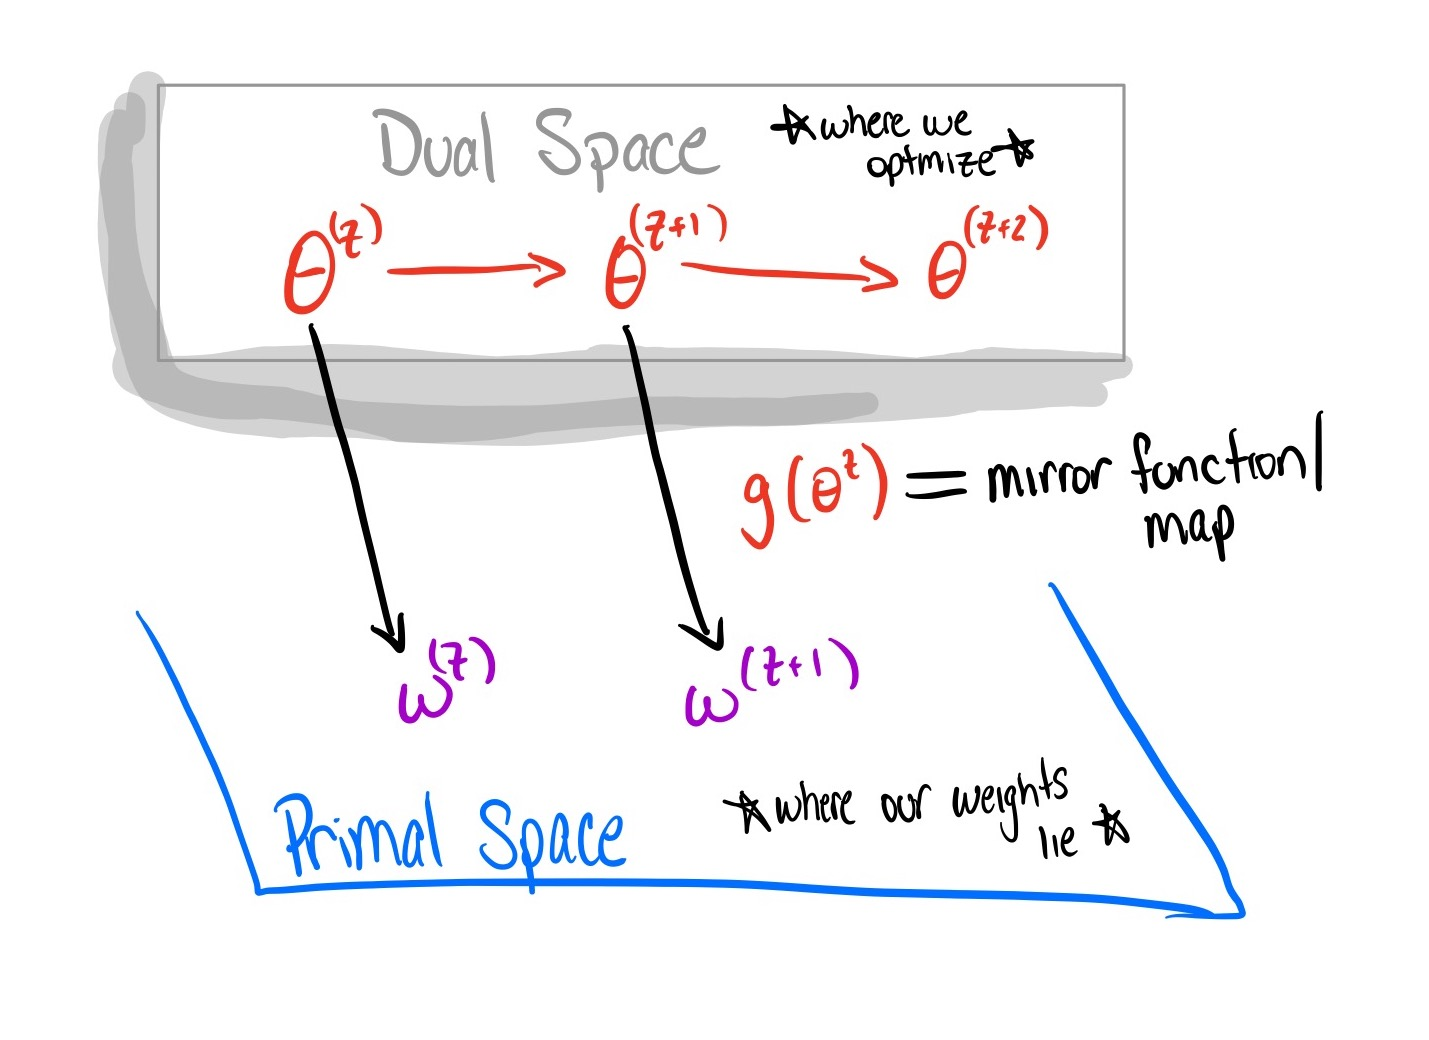
\includegraphics[width=0.7\textwidth]{figs/Page1.jpg}
    \caption{Online Mirror Descent visualization (adapted from slides)}
    \label{fig:omd}
\end{figure}

Lastly, we can see that different choices of regularization leads to different mirror functions (Eq. \ref{eq:7}), which allows us to take better advantage of the geometry of the solution space, consequently leading to different algorithms!

\subsection{Duality}
\label{sec:duality}

\subsubsection{Convex Conjugate}
To fully understand OMD, we must first understand convex conjugates, which are commonly known as a conjugate function, Fenchel dual/conjugate/transform, or Legrande transform. Here we assume only smooth convex functions, however convex conjugates can take on other non smooth or convex forms. The equation for a convex conjugate is as follows:


\begin{align}
\label{eq:8}
    \psi^*(\theta) = \max\limits_{\textbf{w}} (\langle \theta, w \rangle - \psi(w))
\end{align}

To better understand the primal and dual spaces of OMD, it is important to know a function can be parameterized in two ways:

\begin{enumerate}
    \item \textbf{Primal:} function / value parameterization:
    $\{\psi(w), w\}$
    \item \textbf{Dual:} intercept / slope parameterization: 
    $\{b(\theta), \theta\}$
\end{enumerate}


As mentioned in a previous section, we compute a mirror function $g(\theta)$ for each time step, which we use to transform from the primal to dual space, and back again. The primal space is the one we are interested in and want to compute the parameters of. However, it may be easier to optimize in the dual space. OMD allows us the functionality to do so. See the appendix for more insight into conjugate functions.




The convex conjugate exhibits some interesting properties:
\begin{enumerate}
    \item The gradient of the conjugate function is the optimal point on the function
    
    \begin{align}
    \label{eq:9}
        \nabla_\theta \psi^*(\theta) = \frac{\partial \psi^*(\theta)}{\partial \theta} = w^*
    \end{align}
    
    \item Maximizer function
    
    \begin{align}
    \label{eq:10}
        w^* = \text{arg} \max\limits{\textbf{w}} (\langle \theta, w \rangle - \psi(w))
    \end{align}
    
    \item Slope function
    
    \begin{align}
    \label{eq:11}
        \nabla_w \psi(w) = \frac{\partial \psi^*(w)}{\partial w}|_{w=w^*} = \theta
    \end{align}
    
    
    \item Fenchel-Young Inequality (lower bound on conjugate function)
    
    \begin{align}
    \label{eq:12}
        \psi^* (\theta) \geq (\langle w, \theta \rangle - \psi(w))
    \end{align}
    
 
\end{enumerate}


\subsubsection{Bregman Divergence}
In the general case, the Bregman Divergence is an approximation error between two points, according to some proximity function $\psi$. What exactly this divergence is is dependent on how you define $\psi$. In the specific case of OMD, this proximity function is the regularizer. The definition of Bregman Divergence is as follows:

\begin{align}
\label{eq:13}
    D_{\psi}(w||u) = \psi(w) - \psi(u) - \nabla \psi(u)^T(w-u)
\end{align}















\subsection{Generic Regret Bound of OMD}
\label{sec:regret}
Using concepts from Sec. \ref{sec:omd} and Sec. \ref{sec:duality}, we will now derive the regret bound for OMD. Before we do so, we need to know the concept of telescoping:

\definition{A telescoping series is a series whose partial sums eventually only have a
fixed number of terms after cancellation, i.e., its general term is usually of the form $t_n = a_n - a_{n+1}$.}

\normalfont
This concept can be used to make an expression a telescoping series by adding and subtracting the same term such that the expression can now be expressed as a partial sum.

We will now prove below the generic upper regret bound of OMD. Recall that regret is defined as:
\begin{align}
\label{eq:14}
    R(\textbf{u}) = \sum_{t=1}^{T} \textbf{w}^{(t)} \cdot \textbf{z}^{(t)} - \textbf{u} \cdot \textbf{z}^{(t)}
\end{align}

\theorem{(Regret bound of OMD) 
\begin{align}
R(\textbf{u}) \leq \psi(\textbf{u}) - \psi(\textbf{w}^{(1)}) + \sum_{t=1}^{T} D_{\psi^{*}} (-\textbf{z}^{(1:t)} \Vert -\textbf{z}^{(1:t-1)})
\end{align}

\label{theorem:regretbound}

The regret of OMD is upper bounded by the total sum of the difference between regularization function and the sum of all of the Bregman Divergence under the convex conjugate of the regularization function.}

\proof{The loss of an arbitrary vector \textbf{u} is given by:
\begin{align*}
  &\psi(\textbf{u}) + \sum_{t=1}^{T} \textbf{u} \cdot \textbf{z}^{(t)}\\
  &= \psi(\textbf{u}) - \textbf{u} \cdot \bm\theta^{(T+1)} \;\;\; (\text{Using Eq. \ref{eq:2} and Eq. \ref{eq:3}})  
\end{align*}

Applying Fenchel-Young Inequality (Eq. \ref{eq:12}):
\begin{align}
\label{eq:16}
    \psi(\textbf{u}) - \textbf{u} \cdot \bm\theta^{(T+1)} \geq -\psi^{*}(\bm\theta^{(T+1)})
\end{align}

Applying telescoping, we get:
\begin{align*}
-\psi^{*}(\bm\theta^{(T+1)}) &= -\psi^{*}(\bm\theta^{(T+1)}) -\psi^{*}(\bm\theta^{(T)}) + \psi^{*}(\bm\theta^{(T)}) - \cdots - \psi^{*}(\bm\theta^{(1)}) + \psi^{*}(\bm\theta^{(1)}) \\
&= - \psi^{*}(\bm\theta^{(1)}) - \sum_{t=1}^{T}\left(\psi^{*}(\bm\theta^{(t+1)}) -\psi^{*}(\bm\theta^{(t)})\right) \;\;\; (\text{Sum over shifted time steps})
\end{align*}
Using Eq. \ref{eq:13}, we get:
\begin{align}
\label{eq:17}
-\psi^{*}(\bm\theta^{(T+1)}) = - \psi^{*}(\bm\theta^{(1)}) - \sum_{t=1}^{T}\left(\nabla \psi^{*}(\bm\theta^{(t)})\cdot(\bm\theta^{(t+1)}-\bm\theta^{(t)}) + D_{\psi^{*}}(\bm\theta^{(t+1)}||\bm\theta^{(t)}) \right)
\end{align}
The first term of Eq. \ref{eq:17} ($- \psi^{*}(\bm\theta^{(1)})$) can be written as $\psi(\textbf{w}^{(1)})$ as shown below:
\begin{align*}
\psi^{*}(\bm\theta^{(1)}) &= \psi^{*}(\textbf{z}^{(0)}) \;\;\; (\text{Using Eq. \ref{eq:3}})\\
&= \psi^{*}(\textbf{0}) \;\;\; (\text{From initialization})\\
&= \max\limits_{\textbf{w}} \{ \langle \textbf{w}, \textbf{0} \rangle - \psi(\textbf{w}) \} \;\;\; (\text{Using Eq. \ref{eq:8}})\\
&= \max\limits_{\textbf{w}} \{ 0 - \psi(\textbf{w}) \} \;\;\; (\text{Compute dot product})\\
&= -\min\limits_{\textbf{w}} \{ \psi(\textbf{w}) \} \;\;\; (\text{Convert to min problem})
\end{align*}
At $t=1$, the minimizer of cumulative loss is the primal iterate at step 1 (`the one-step look ahead cheater', discussed while deriving the intermediate regret bound of Algo. \ref{algo:ftrl}). Thus we get:
\begin{align}
\label{eq:18}
  \psi^{*}(\bm\theta^{(1)})  = -\psi(\textbf{w}^{(1)})
\end{align}
Eq. \ref{eq:17} can be further reduced:
\begin{align*}
-\psi^{*}(\bm\theta^{(T+1)}) &= - \psi^{*}(\bm\theta^{(1)}) - \sum_{t=1}^{T}\left(\nabla \psi^{*}(\bm\theta^{(t)})\cdot(\bm\theta^{(t+1)}-\bm\theta^{(t)}) + D_{\psi^{*}}(\bm\theta^{(t+1)}||\bm\theta^{(t)}) \right) \;\;\; (\text{From Eq. \ref{eq:17}})\\
&= \psi(\textbf{w}^{(1)}) - \sum_{t=1}^{T}\left(\nabla \psi^{*}(\bm\theta^{(t)})\cdot(\bm\theta^{(t+1)}-\bm\theta^{(t)}) + D_{\psi^{*}}(\bm\theta^{(t+1)}||\bm\theta^{(t)}) \right) \;\;\; (\text{Using Eq. \ref{eq:18}})\\
&= \psi(\textbf{w}^{(1)}) - \sum_{t=1}^{T}\left(\textbf{w}^{(t)}\cdot(\bm\theta^{(t+1)}-\bm\theta^{(t)}) + D_{\psi^{*}}(\bm\theta^{(t+1)}||\bm\theta^{(t)}) \right) \;\;\; (\text{Using Eq. \ref{eq:9}})\\
&= \psi(\textbf{w}^{(1)}) - \sum_{t=1}^{T}\left(\textbf{w}^{(t)}\cdot(-\textbf{z}^{(1:t)}+\textbf{z}^{(1:t-1)}) + D_{\psi^{*}}(-\textbf{z}^{(1:t)}||-\textbf{z}^{(1:t-1)}) \right) \;\;\; (\text{Using Eq. \ref{eq:3}})\\
&= \psi(\textbf{w}^{(1)}) - \sum_{t=1}^{T}\left(\langle \textbf{w}^{(t)}, -\textbf{z}^{(t)} \rangle + D_{\psi^{*}}(-\textbf{z}^{(1:t)}||-\textbf{z}^{(1:t-1)}) \right)
\end{align*}
Moving negative out of the sum:
\begin{align}
\label{eq:19}
-\psi^{*}(\bm\theta^{(T+1)}) &= \psi(\textbf{w}^{(1)}) + \sum_{t=1}^{T}\left(\langle \textbf{w}^{(t)}, \textbf{z}^{(t)} \rangle - D_{\psi^{*}}(-\textbf{z}^{(1:t)}||-\textbf{z}^{(1:t-1)}) \right)
\end{align}
Combining Eq. \ref{eq:16} and Eq. \ref{eq:19}, we get:
\begin{align*}
\psi(\textbf{u}) - \textbf{u} \cdot \bm\theta^{(T+1)} &\geq \psi(\textbf{w}^{(1)}) + \sum_{t=1}^{T}\left(\langle \textbf{w}^{(t)}, \textbf{z}^{(t)} \rangle - D_{\psi^{*}}(-\textbf{z}^{(1:t)}||-\textbf{z}^{(1:t-1)}) \right)\\
-\psi(\textbf{u}) + \textbf{u} \cdot \bm\theta^{(T+1)} &\leq -\psi(\textbf{w}^{(1)}) - \sum_{t=1}^{T}\left(\langle \textbf{w}^{(t)}, \textbf{z}^{(t)} \rangle - D_{\psi^{*}}(-\textbf{z}^{(1:t)}||-\textbf{z}^{(1:t-1)}) \right) \;\;\; (\text{Multiplying by negative sign})\\
-\psi(\textbf{u}) + \langle \textbf{u}, -\textbf{z}^{(1:T)} \rangle &\leq -\psi(\textbf{w}^{(1)}) - \sum_{t=1}^{T}\left(\langle \textbf{w}^{(t)}, \textbf{z}^{(t)} \rangle - D_{\psi^{*}}(-\textbf{z}^{(1:t)}||-\textbf{z}^{(1:t-1)}) \right) \;\;\; (\text{Using Eq. \ref{eq:3}})\\
-\psi(\textbf{u}) + \langle \textbf{u}, -\textbf{z}^{(1:T)} \rangle &\leq -\psi(\textbf{w}^{(1)}) - \sum_{t=1}^{T}\langle \textbf{w}^{(t)}, \textbf{z}^{(t)} \rangle +\sum_{t=1}^{T} D_{\psi^{*}}(-\textbf{z}^{(1:t)}||-\textbf{z}^{(1:t-1)}) \;\;\; (\text{Multiply through sign})
\end{align*}


Rearranging terms:
\begin{align*}
 \sum_{t=1}^{T}\langle \textbf{w}^{(t)}, \textbf{z}^{(t)} \rangle + \langle \textbf{u}, -\textbf{z}^{(1:T)} \rangle &\leq \psi(\textbf{u}) -\psi(\textbf{w}^{(1)}) +\sum_{t=1}^{T} D_{\psi^{*}}(-\textbf{z}^{(1:t)}||-\textbf{z}^{(1:t-1)})\\
  \sum_{t=1}^{T}\langle \textbf{w}^{(t)}, \textbf{z}^{(t)} \rangle + \sum_{t=1}^{T}\langle \textbf{u}, -\textbf{z}^{(t)} \rangle &\leq \psi(\textbf{u}) -\psi(\textbf{w}^{(1)}) +\sum_{t=1}^{T} D_{\psi^{*}}(-\textbf{z}^{(1:t)}||-\textbf{z}^{(1:t-1)}) \;\;\; (\text{Using Eq. \ref{eq:2}})\\
  \sum_{t=1}^{T}\langle \textbf{w}^{(t)}, \textbf{z}^{(t)} \rangle - \langle \textbf{u}, \textbf{z}^{(t)} \rangle &\leq \psi(\textbf{u}) -\psi(\textbf{w}^{(1)}) +\sum_{t=1}^{T} D_{\psi^{*}}(-\textbf{z}^{(1:t)}||-\textbf{z}^{(1:t-1)}) \;\;\; (\text{Combining sums})\\
    \sum_{t=1}^{T}\textbf{w}^{(t)} \cdot \textbf{z}^{(t)} - \textbf{u} \cdot \textbf{z}^{(t)} &\leq \psi(\textbf{u}) -\psi(\textbf{w}^{(1)}) +\sum_{t=1}^{T} D_{\psi^{*}}(-\textbf{z}^{(1:t)}||-\textbf{z}^{(1:t-1)}) \;\;\; (\text{Changing notations})\\
    R(\textbf{u}) &\leq \psi(\textbf{u}) -\psi(\textbf{w}^{(1)}) +\sum_{t=1}^{T} D_{\psi^{*}}(-\textbf{z}^{(1:t)}||-\textbf{z}^{(1:t-1)}) \;\;\; (\text{Using Eq. \ref{eq:14}})\\
\end{align*}

We have thus proved the generic upper regret bound of OMD. 


}
\section{Appendix}

\subsection{Geometrical Interpretation of Conjugate Function}

\begin{figure}[H]
    \centering
    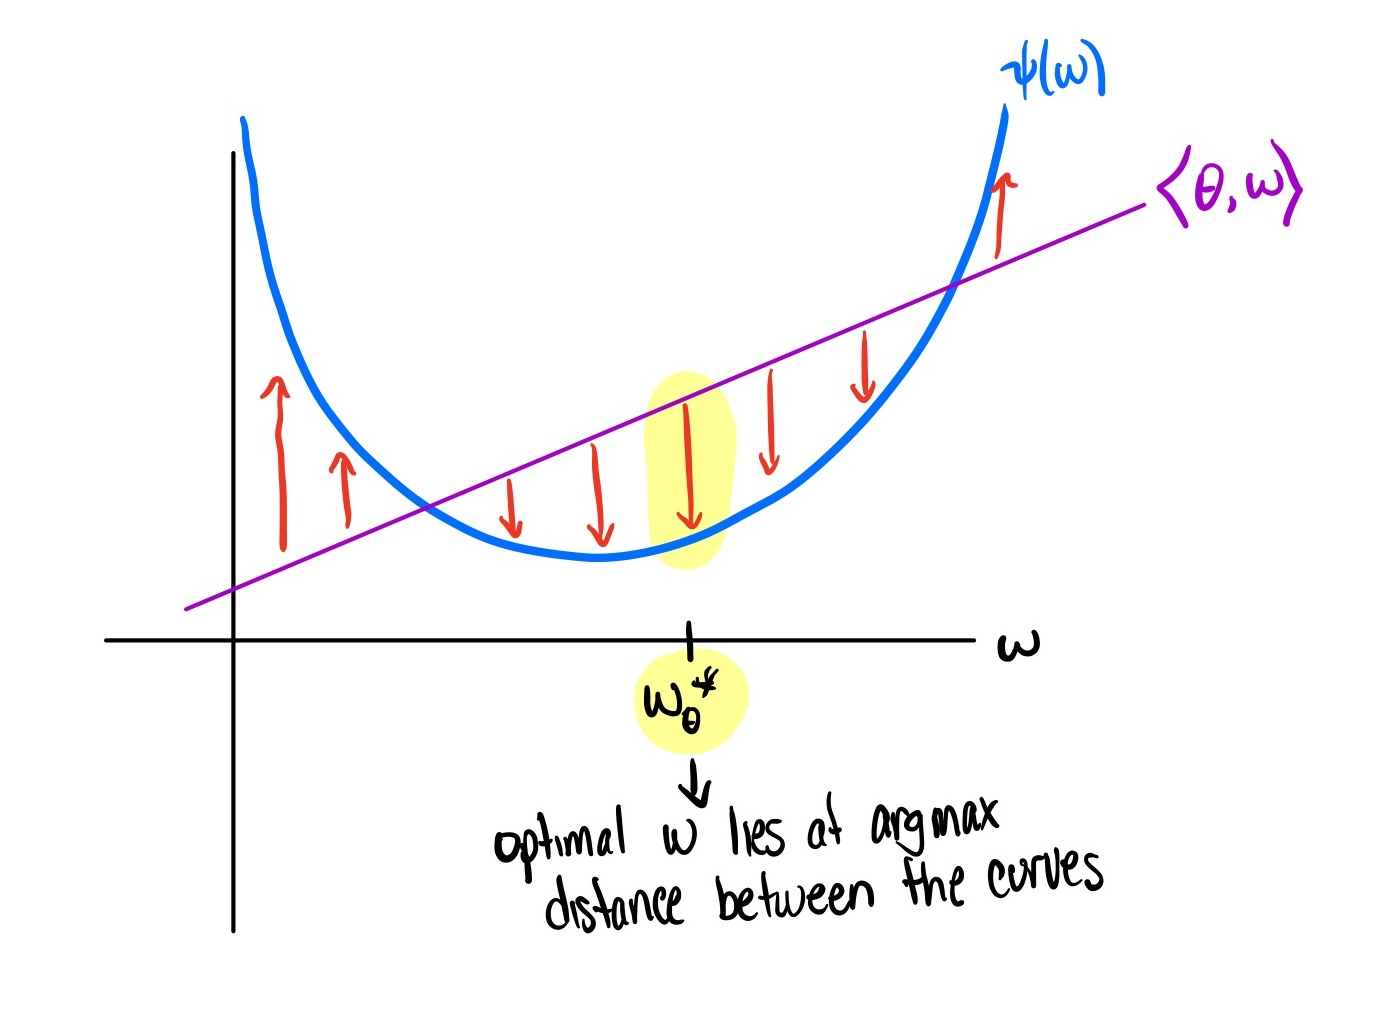
\includegraphics[width=0.5\textwidth]{figs/Page2.jpg}
    \caption{Conjugate Function Geometry (adapted from slides)}
    \label{fig:conj}
\end{figure}

To get a better idea of conjugate functions, Figure (3) shows a geometrical interpretation of the conjugate function. In this, we have our primal function, a line $\langle \theta, w \rangle$ that passes through the origin with slope $\theta$. The dual parameterization is $\psi(w)$ parameterized by $w$, in which we are trying to find the minimum $w_{\theta}^*$ of. Consider the difference between the primal and dual parameterizations. From the figure, we can see that the maximum difference actually occurs at the location where the tangent line meets $\psi(w)$, and also has a slope of $\theta$. In other words, it is parallel to $\langle \theta, w \rangle$. The conjugate function at $\psi (\theta)$ is the intercept of the tangent line, which is therefore equivalent to the maximum difference of $\langle \theta, w \rangle - \psi(w)$.


\subsection{Geometrical Interpretation of Bregman Divergence}

\begin{figure}[H]
    \centering
    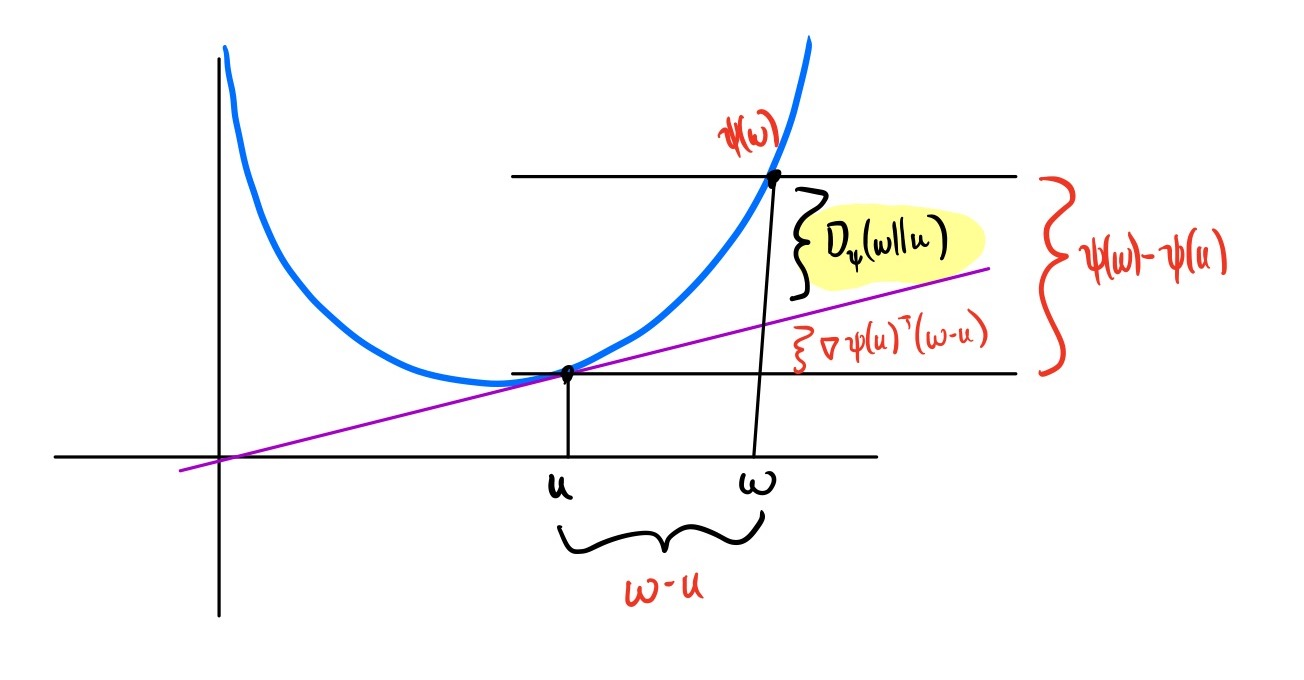
\includegraphics[width=0.7\textwidth]{figs/Page3.jpg}
    \caption{Bregman Divergence Geometry (adapted from slides)}
    \label{fig:bregman}
\end{figure}

Figure (4) shows a geometric interpretation of the Bregman Divergence that may be more intuitive to understand. Given two points $u$ and $v$, we can calculate their difference as well as their difference in values on the proximity function $\psi$, as shown on the bottom and right sides of the figure, respectively. As we can observe, the Bregman Divergence estimates the approximate error between the points by finding the difference between (1) the difference of their function values $\psi(w)$ - $\psi(u)$ and (2) the first order approximation of $\psi(w)$, $\nabla \psi (u)^T(w-u)$. This will come in handy as we form the regret bound for OMD.


%This section provides any relevant background material that was not covered in the lectures, but was found to be useful for understanding the material. 
%For example, derivations, theory underlying techniques employed, etc. 

%Additionally, this section can summarizes applications or extensions of these techniques found in the literature. 


\section*{References}

[1] Wikipedia contributors. Bregman divergence -- Wikipedia, the free encyclopedia, 2022. [Online; accessed 16-Feb-2022].

[2] Wikipedia contributors. Convex conjugate -- Wikipedia, the free encyclopedia, 2022. [Online; accessed 16-Feb-2022].
%Include your references here. Please cite any resources you found useful.	
%Populate the refs.bib file or list your references manually. Be consistent in formatting!
{
\bibliography{refs}
\bibliographystyle{abbrv}
}

\end{document} % Done!

